\chapter{Conclusiones\label{sec:conclusiones}}

\section{Introducción}
En este capítulo se expondrán las conclusiones extraídas como resultado del proyecto, además de los problemas encontrados a la hora de realizar el mismo y la forma en que se han abordado.

Para su realización ha sido necesario un curso de formación para el aprendizaje sobre el uso de las herramientas pertenecientes al ecosistema, así como la instalación manual del mismo en los equipos de mi domicilio que han realizado la función de clúster. 

La proyección de este ha requerido de tres meses para el planteamiento, implementación y resolución; desarrollando para ello varios \textit{scripts} y aplicaciones que han sido necesarios para la resolución de los diferentes problemas, más un informe final con las recomendaciones para el supuesto cliente en el que se ha basado este desarrollo.

\clearpage
\section{Conclusiones}
La primera fase de este proyecto consistió en la selección de las herramientas que se utilizarían, para ello se decidió prescindir de las más antiguas, aunque actualmente se encuentren en proyectos en producción, a favor de \textit{Apache Spark} que posee el potencial no solo de sustituirlas sino de ofrecer mejor rendimiento sobre el mismo \textit{hardware}.

La instalación del sistema \textit{big data} y su adaptación al \textit{hardware} disponible requirió dos semanas; posteriormente se establecieron los objetivos para la demostración del uso de esta tecnología en un proyecto real.

La siguiente fase consistió en la selección y estudio de las fuentes de datos disponibles, así como establecer el valor y veracidad de los mismos. Algunos de los problemas que se encontraron durante esta fase fue por un lado que algunas de las empresas habían establecido una \gls{API} de pago y por otro que los datos proporcionados eran intencionadamente incompletos. Para sortear estos inconvenientes se hizo uso de la \gls{API} gratuita disponible y cruzando los datos para asegurar tanto el linaje como su veracidad.

Por desgracia, al ser un trabajo hipotético no se ha tenido acceso a los datos internos de la empresa que habría supuesto uno de los pilares principales sobre los que trabajar. Ver figura \ref{DataSources} 

Además, la mayoría de los datos eran semiestructurados o directamente no poseían estructura alguna. Para resolver esto se utilizaron \textit{parsers} y un filtrado sumario, siendo recomendable la realización de un proyecto de \textit{Data Text Mining} para la extracción de información, pero del que se prescindió debido a las limitaciones de tiempo para el desarrollo del proyecto.

\begin{figure}[htp!]
	\centering
	\caption{Esquema de orígenes de datos del proyecto}
	\label{DataSources}
	\vspace{5pt}
	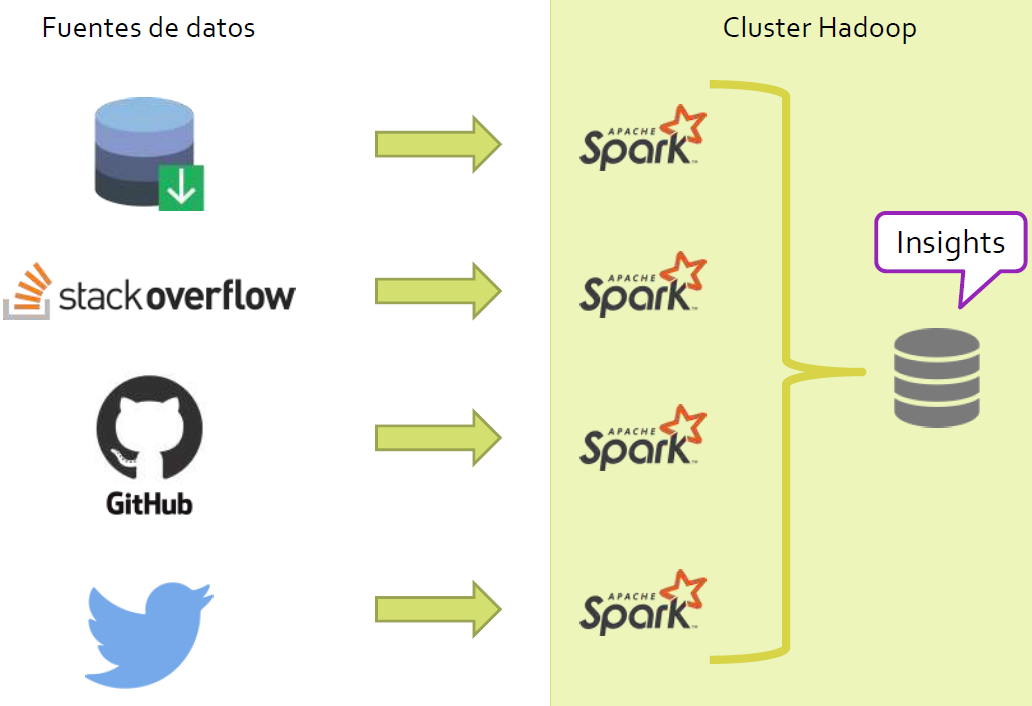
\includegraphics[scale=0.41]{graphics/dataSources}
\end{figure}

\clearpage
\section{Informe final}
\subsection{Lenguajes populares}
El primer \textit{insight} planteado corresponde a los lenguajes populares, para ello se han analizado las plataformas de Stack Overflow \cite{stackoverflow} (ver apartado \ref{sec:stackoverflow}) y GitHub \cite{github} (ver apartado \ref{sc:github}), que nos proporcionan información sobre qué preguntan los programadores y en qué trabajan respectivamente.

Como se puede observar en la figura \ref{HistGitHub} referente a la analítica de GitHub de los últimos tres años hay varios lenguajes de sobra conocidos en el sector, pero han aparecido algunos como Rust, Go, Scala o Kotlin que han adquirido una gran importancia en relativamente poco tiempo, equiparándose o superando lenguajes con varios años de bagaje, por lo que sería altamente recomendable la realización de cursos relacionados con estos lenguajes debido a su potencial y rápida aceptación por los profesionales del sector.

En la figura \ref{HistStof} se puede observar cómo algunos de los lenguajes han tenido una menor incidencia en el último año con respecto a otros anteriores, con la salvedad de Python, el cual ha aumentado su presencia en este último año pese a ser un lenguaje establecido, por lo que se prevee un relanzamiento de este en los próximos años.

En definitiva la recomendación en función de los datos sería mantener los cursos en Javascript, Java, PHP, C++, Android e Ios y aumentar o crear cursos sobre Rust, Go, Scala, Kotlin y Python.
\begin{figure}[htp!]
	\centering
	\caption{Histórico Stack Overflow}
	\label{HistStof}
	\vspace{5pt}
	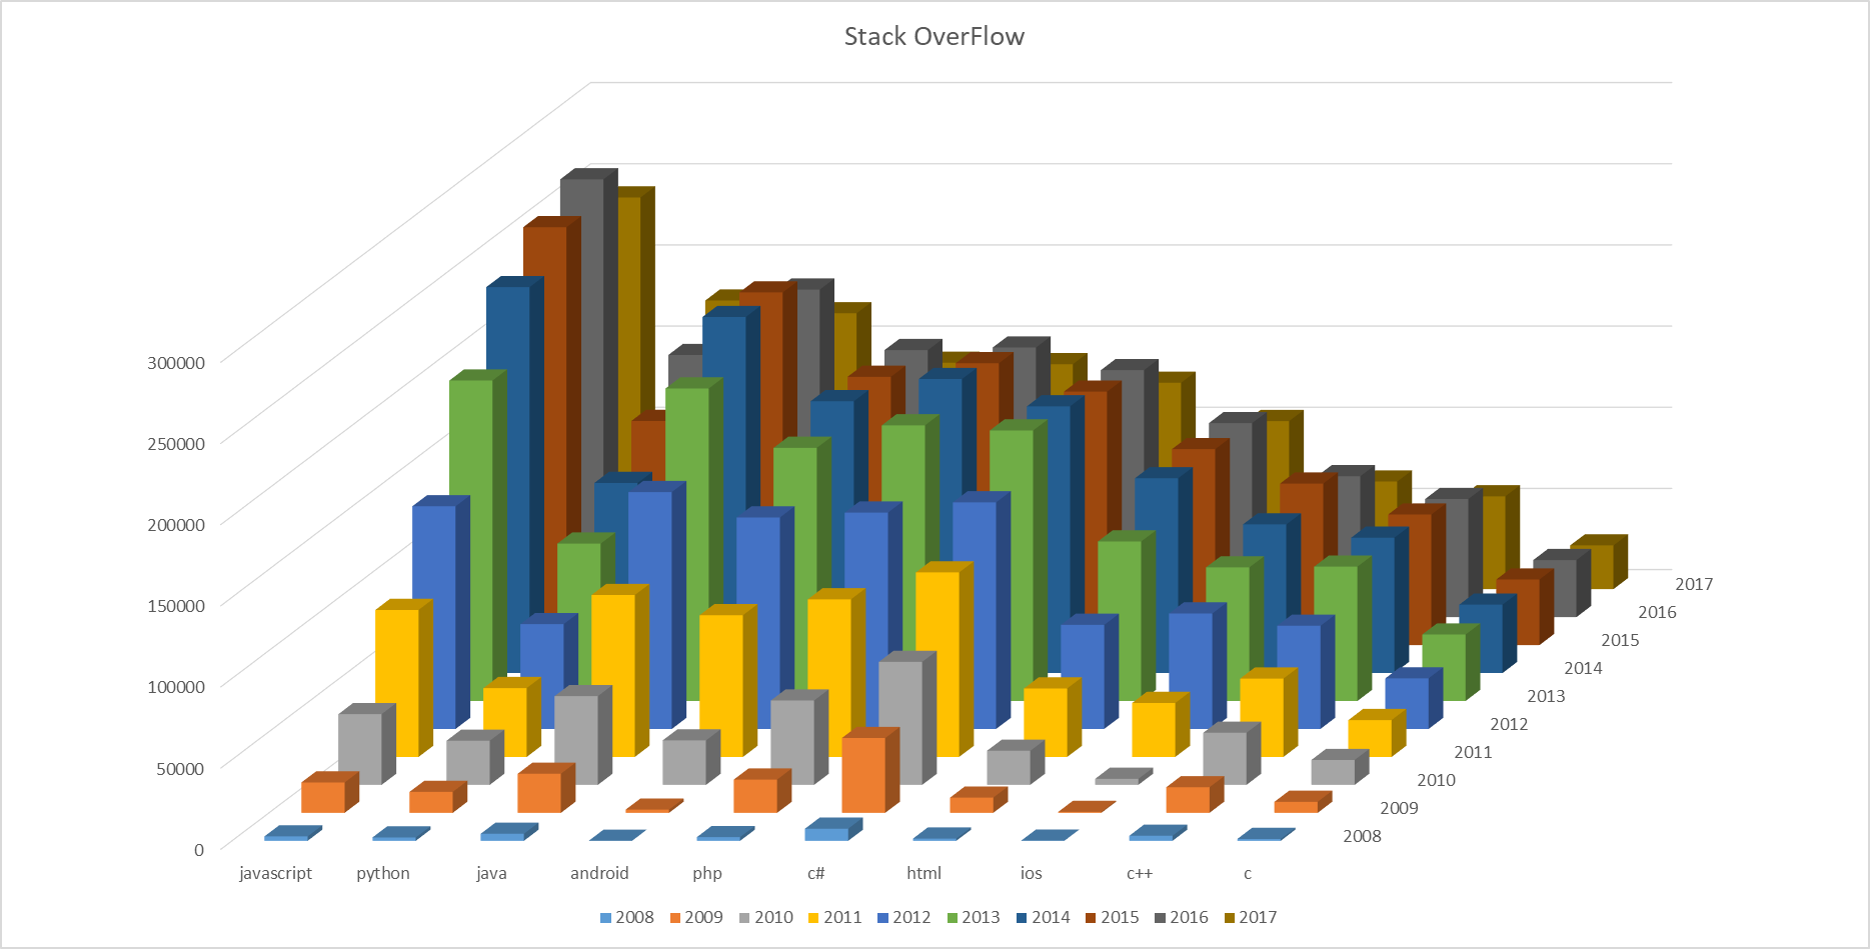
\includegraphics[scale=0.55]{graficas/stofHist}
\end{figure}
\begin{figure}[htp!]
	\centering
	\caption{Histórico de GitHub}
	\label{HistGitHub}
	\vspace{5pt}
	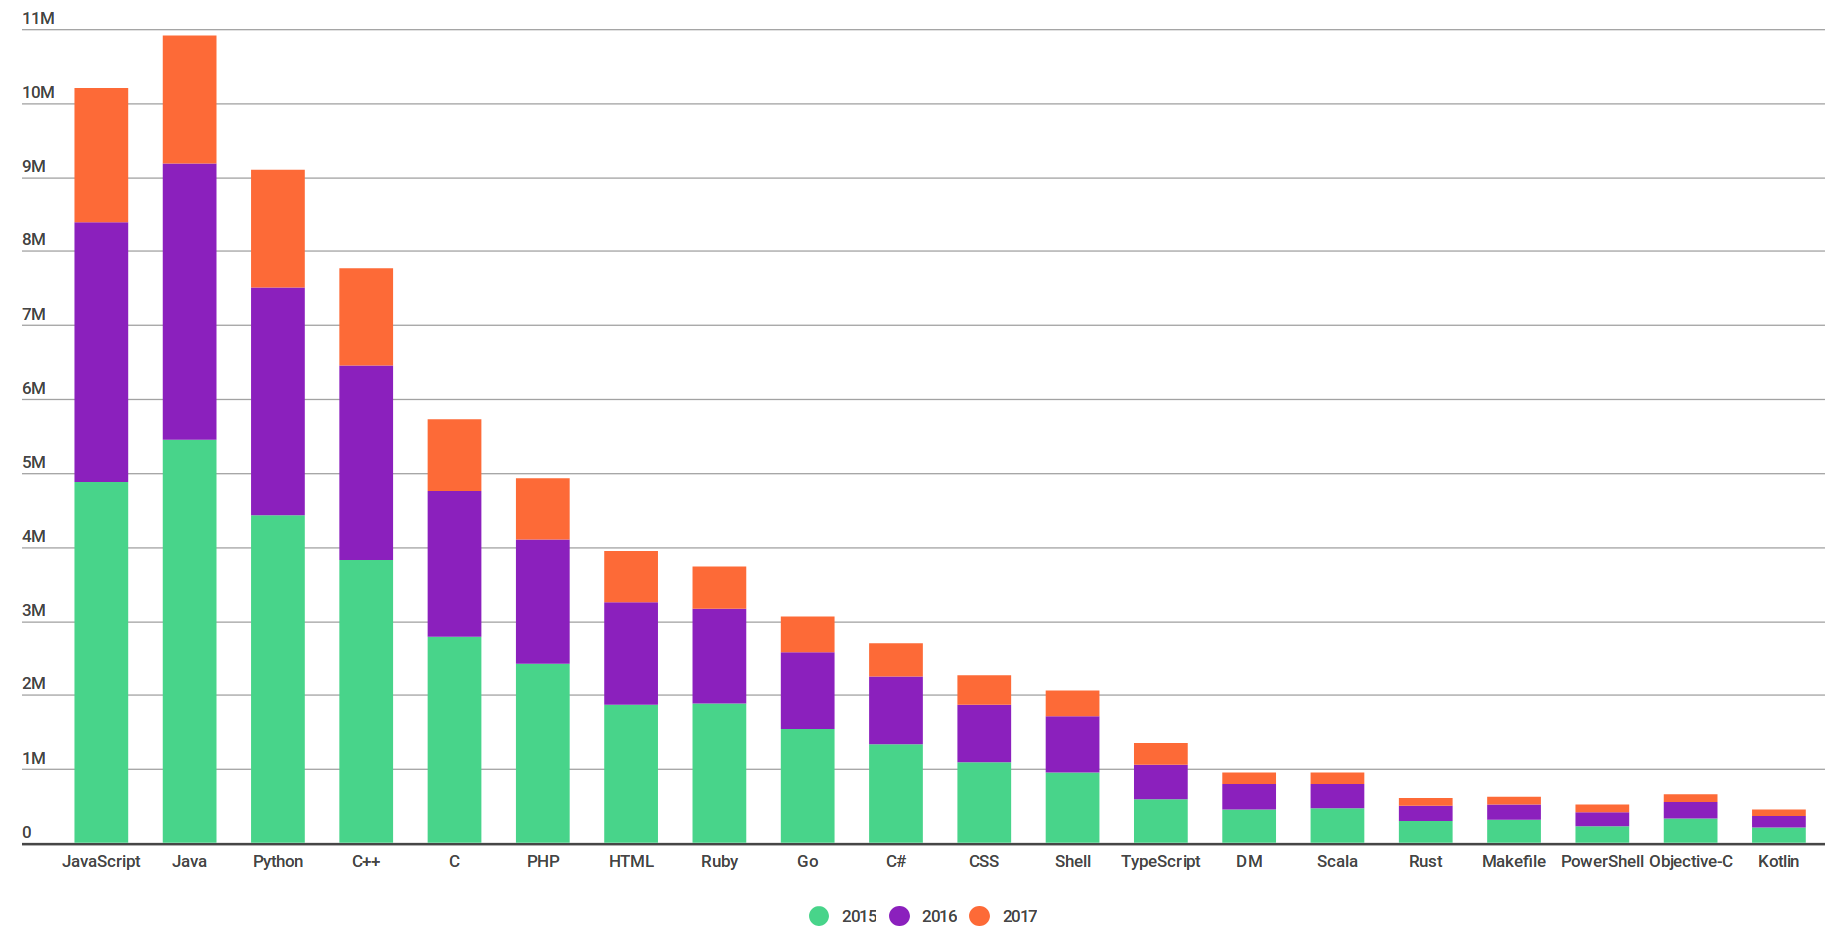
\includegraphics[scale=0.25]{graficas/githubBarTotal}
\end{figure}


\clearpage
\subsection{Regionalización de la empresa}
Otro de los \textit{insight} que solicitaba la empresa era un análisis sobre los países en los que enfocarse en caso de decidir regionalizar los cursos.
\begin{figure}[htp!]
	\centering
	\caption{Mapamundi de incidencia de programadores por país}
	\label{Mapamundi}
	\vspace{5pt}
	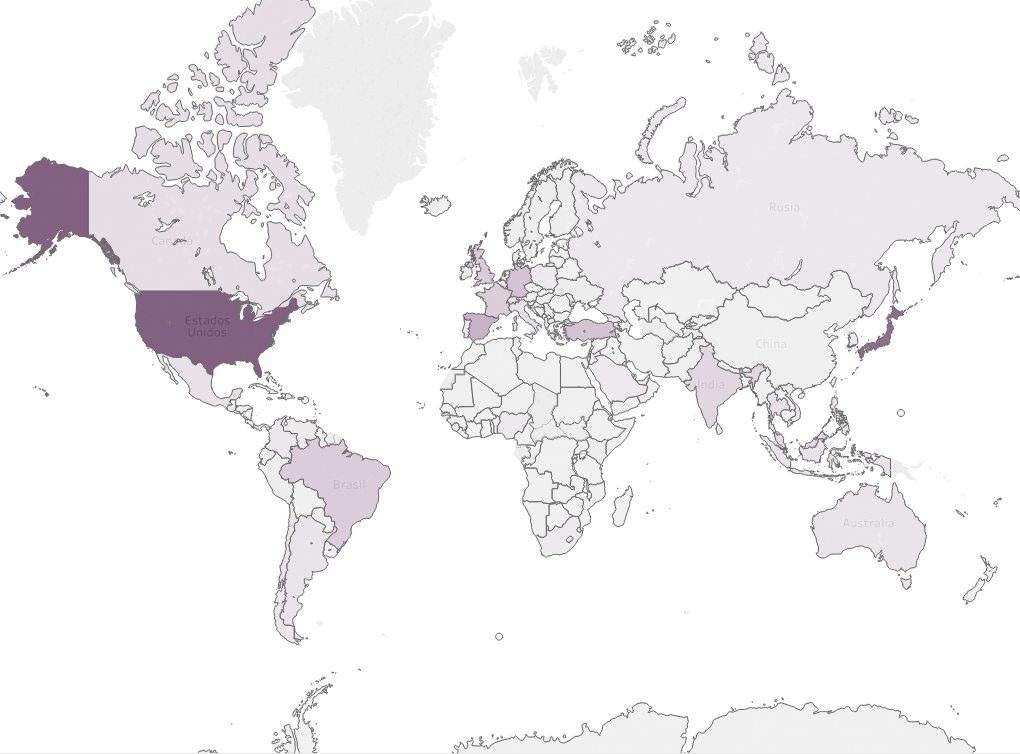
\includegraphics[scale=0.63]{graficas/CorrectMap}
\end{figure}

En la figura \ref{Mapamundi} se puede observar que la mayor incidencia se encuentra en Estados Unidos y Japón, seguido por Brasil, España, Francia, Turquía e India. La recomendación en este punto sería aumentar la presencia en estos dos países principalmente y luego expandirse hacia Europa y Sudamérica. 

Estos datos han sido extraídos de Twitter \cite{twitter}, este punto es importante ya que explica la ausencia completa de datos en China, país donde se usa la plataforma Weibo \cite{weibo} en sustitución de Twitter. Pero es un mercado de fácil acceso desde Japón sin tener que establecerse en el país.

\clearpage	
\subsection{Idioma vehicular}
\begin{figure}[htp!]
	\centering
	\caption{Gráfica orientativa sobre el uso de idiomas}
	\label{Idiomas}
	\vspace{5pt}
	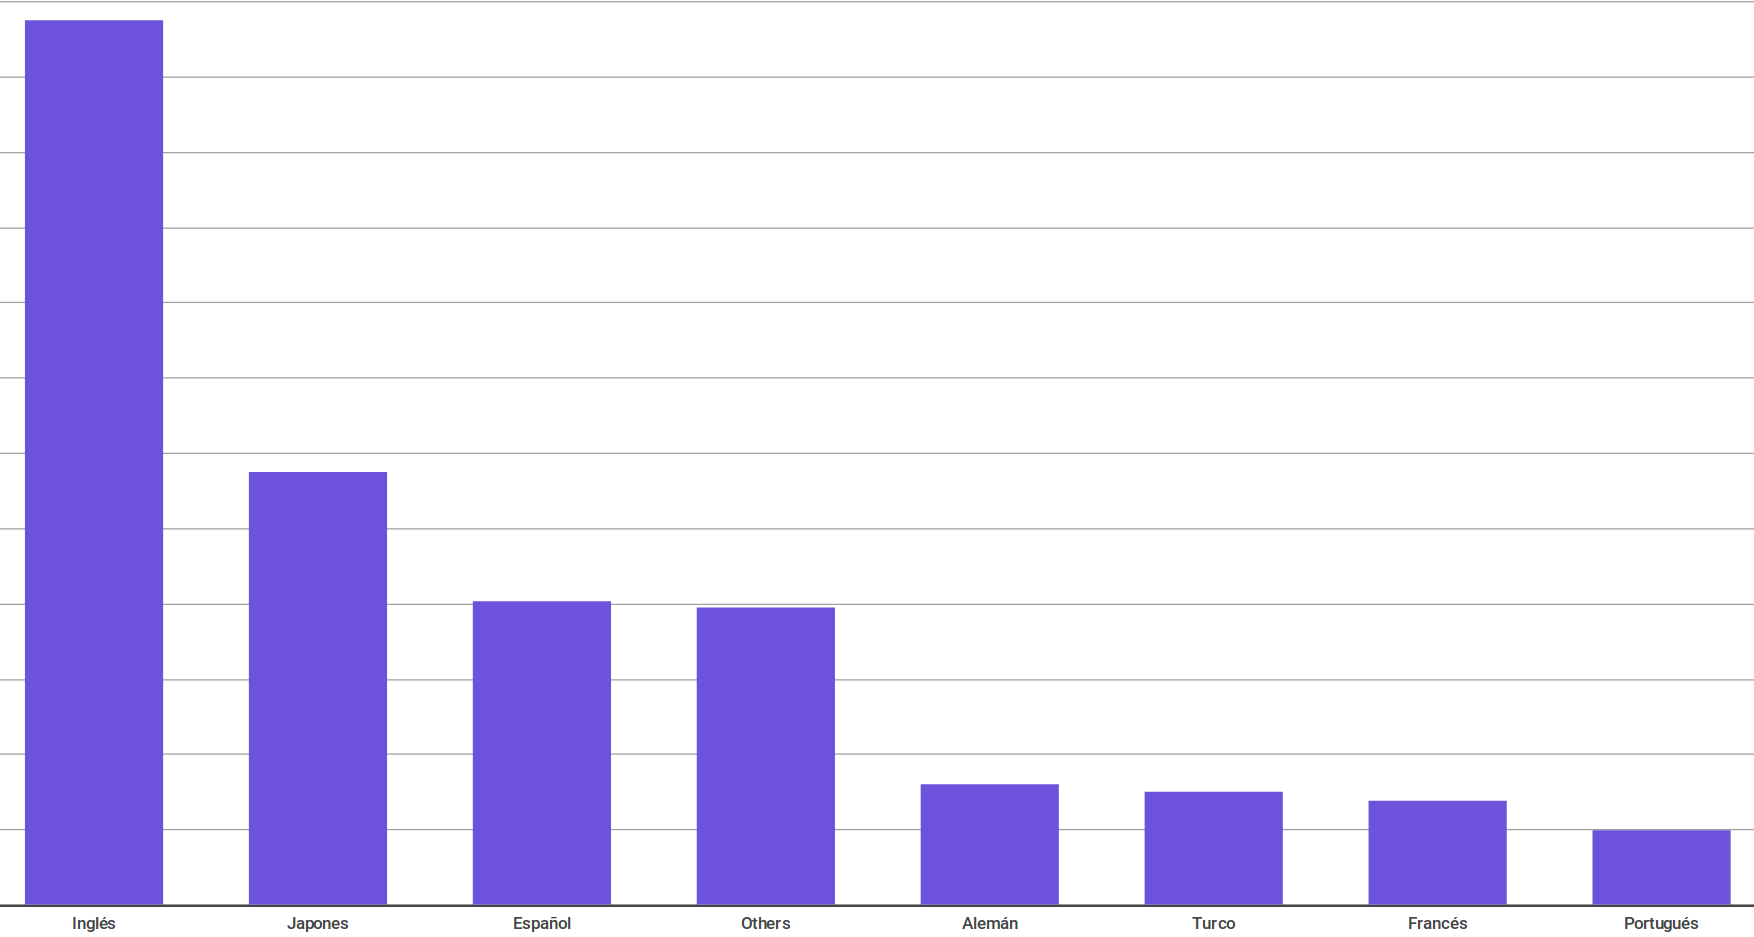
\includegraphics[scale=0.355]{graficas/LenguajesBarCorrect2}
\end{figure}

En este punto no se aprecian grandes sorpresas, el idioma principal es el inglés que además es la segunda lengua de la mayoría de los profesionales del sector, por lo que se recomienda el uso de esta para los cursos. Además, el segundo puesto lo ocupa el japones seguido del español, este primer idioma sería interesante a la hora de acercarse a una población con gran impacto tecnológico y el segundo debido al gran volumen de hispanohablantes.

El resto de idiomas tiene un impacto mucho menor, teniendo los idiomas minoritarios en conjunto un impacto similar al español.

La recomendación sería utilizar el inglés como idioma principal, asegurando la existencia de subtítulos o contenido en japonés y español para maximizar la cartera de clientes potenciales manteniendo un bajo costo por curso.